\section{Background}
% Section outline
% Overall summary of section - ~1 sentence per major topic
% ~1 Paragraph for each major topic
This section begins with an overview of some existing robotic arms that are about the same size as a fully assembled arm from our kit will be. Next we discuss some existing modular robotic arms. Finally, we highlight how our kit will be different from the discussed prior art.

\subsection{Robot Arms Currently in Use}
There are a plethora of industrial robotic arms. Since our kit will be relatively small compared to most industrial arms, we will begin with an overview of existing desktop industrial arms. Arms that fit this description have a reach of less than 1000mm. Industrial robot arms typically cost between \$50,000 and \$80,000 new and \$25,000 and \$40,000 used \cite{RobotWorx}. Some manufacturers of these industrial arms include ABB Robotics, Universal Robots, and KUKA Robotics.

\subsubsection{ABB Robotics}
ABB Robotics makes many small industrial arms. The ABB IRB 120 boasts a 580mm reach, 3kg payload, and 25kg weight. It has 6 degrees of freedom and can be mounted at any angle. The ABB IRB 1200 comes in two varieties, one with a reach of 703mm reach and 7kg payload, and one with a 901mm reach and 5kg payload. Both of these arms have 6 degrees of freedom. The weights are similar at 52kg and 54kg respectively \cite{RobotWorx}.

\subsubsection{Universal Robots}
Universal Robots makes two robot arms in this size range. The UR3 is the smaller of the two with a reach of 500mm, payload of 3kg, and 11kg weight. A step up is the UR5 which has a 850mm reach, 5kg payload, and 18.1kg weight. Both of these arms have 6 degrees of freedom. Universal boasts that these arms are easy to implement and re-implement due to compact and lightweight construction, and simple programming interface \cite{RobotWorx}.

\subsubsection{KUKA AG}
KUKA makes two robot arms in this size range. The KR3 R540 has a reach of 541mm, payload of 3kg, and weight of 26kg. It can be mounted on the floor, wall, or ceiling for added utility. The K5 sixx R650 is larger with a reach of 650mm, payload of 5kg, and weight of 127kg. It can only be mounted on the floor or ceiling. Both of these arms have 6 degrees of freedom \cite{RobotWorx}.

\subsection{Small Industrial Robotic Arm Comparison}
Table \ref{tab:ArmComparison} shows a comparison of all the robotic arms discussed in this section.
\begin{table} [H]
\centering
\begin{tabular}{| l | c | c | c | c |}
\hline
\textbf{Name} & \textbf{Reach (mm)} & \textbf{Payload (kg)} & \textbf{Weight (kg)} & \textbf{Axes} \\
\hline
IRB120 & 580 & 3 & 25 & 6 \\
IRB1200-7/0.7 & 703 & 7 & 52 & 6 \\
IRB1200-5/0.9 & 901 & 5 & 54 & 6 \\
UR3 & 500 & 3 & 11 & 6 \\
UR5 & 850 & 5 & 18.1 & 6 \\
KR3 R540 & 541 & 3 & 26 & 6 \\
K5 sixx R650 & 650 & 5 & 127 & 6 \\
\hline
\end{tabular}
\caption{Comparison of $<$1000mm reach industrial robot arms}
\label{tab:ArmComparison}
\end{table}

\subsection{Modular Arms}
While there are many industrial arms in production, there are very few modular robotic arms. There is one commercially available robotic arm, the Robolink, made by igus. A few modular robot arms have been developed, including the reconfigurable modular manipulator (RMM), made by TRACLabs \cite{RMM}, and a single joint for the Modular Robotic Arm project MQP at WPI \cite{MRA}.

\subsubsection{igus Robolink} 
Robolink is a modular robotic arm kit produced by the plastics manufacturing company igus. The kit contains parts to make an arm that is up to 6 Degrees of Freedom (DOF), with belt driven linkages powered by stepper motors that reside in the base of the robot. Robolink offers 7 individual links, ranging from 1-2 DOF and differing based upon their kind of motion (pivoting, rotating, swiveling). Each link is made of a lightweight and strong plastic or carbon fiber with cables inlaid in them, resulting in a low cost and weight arm. The cables used to control these links are made of a high strength synthetic fiber with has a tensile strength of 4,000N. Separating the actuation of each link from the joint allows the arms to be easily maneuverable with its lightweight and strong joints.

\noindent Purchasers of the kit are able to combine the links in different ways, allowing for a flexible, modular solution to robotic arms. Igus also offers their Robolink software for programming articulated arms that facilitates the programming of individual arms through the use of a simple, intuitive control software. The total cost of a kit to make a 6 DOF arm is \$6000, and buying individual links will cost anywhere from \$370 to \$750 per link. While this price may be low cost compared to other arms such as the ABB robotic arm which can cost up to \$200,000 in total, it is still not low enough for either hobbyists or people interested in learning about robotic arms but prevented from doing so by the high entry cost. In addition to this, the belt system actuating each link requires the user to thread belts attached to the actuators to each link in order to set up the robot. The long assembly time and intricacy also detracts from the idea of a modularity because the time involved in switching configurations can inhibit users from really exploring the different workspaces and combinations this kit can create \cite{igus}. 

\subsubsection{Reconfigurable Modular Manipulator}
The reconfigurable modular manipulator developed by TRACLabs for NASA is a fully modular 7-DOF robot arm. Each joint and end effector have the same connector that provides power and control lines throughout the arm. Internal power and control circuitry take in these lines and convert them into movement. Joints can be swapped out by hand in a matter of seconds. Joints accept position or velocity data from the central communication lines and store physical characteristics about the joints in memory. This robot arm is not commercially available \cite{RMM}.

\subsubsection{Modular Robotic Arm}
This project aimed to close the market gap between inexpensive toy robot arms and expensive professional grade industrial arms. The group aimed to do this by designing a single joint that could be used to assemble a robot arm. Ultimately, a single DOF joint that was heavy, difficult to manufacture, and expensive to produce was designed and constructed. In their future recommendations section, the group stated that the goal of designing a modular robot arm was possible but their design was not the solution \cite{MRA}.

\subsection{Our Robotic Arm System}
Our modular robotic arm kit aims to offer a completely different experience compared to existing products and projects. The system maintains a low cost while providing a versatile platform for beginner engineers or rapid prototyping professionals. This is achieved by avoiding expensive proprietary software and subtractive manufacturing; favoring off-the-shelf parts, 3D-printed structures, and freely available software. Providing custom-built software for controlling the arm creates a plug-and-play environment suitable for most any skill level.


\subsection{Communications}
We looked at several types of communications for the purposes of controlling our robotic arm. These include serial UART, SPI, I2C, and CAN. 
\subsubsection{Controller Area Network}
A controller area network (CAN) is a system for sending data reliably between distinct subsystems with reasonably low danger of transmission errors. CAN buses are widely used in the automotive industry to allow various computerized parts of the car to talk to one another.

% Research begins here?
\subsection{Control board}
We decided to use a control board that consists of a microcontroller, analog-to-digital converter, quadrature encoder counter, motor driver, current sensor, CAN controller, and CAN transceiver. These devices will allow each control board to control one motor.

\noindent Current sensing can be done in multiple ways. The most common way is by using a small resistor in series with the motor and amplifying the voltage across this resistor. This method can cause lots of noise in the system and takes some power from the motor to use. As the value of resistor used increases, so does the power taken from the motor. However, this also causes a larger voltage across the resistor, meaning less amplification is needed and reducing the output noise.

\noindent Other methods of current sensing include hall effect sensors. These sensors measure current non-intrusively by using the motor current to induce a small voltage in a conductor, then amplifying that small voltage and outputting it. The insertion loss caused by these sensors is very small. Since these sensors measure current by induction, they can only measure current in a specific frequency band. Most of these frequencies are DC to some upper limit determined by the physical characteristics of the sensor, usually around 100kHz.

\begin{figure}[H]
\centering
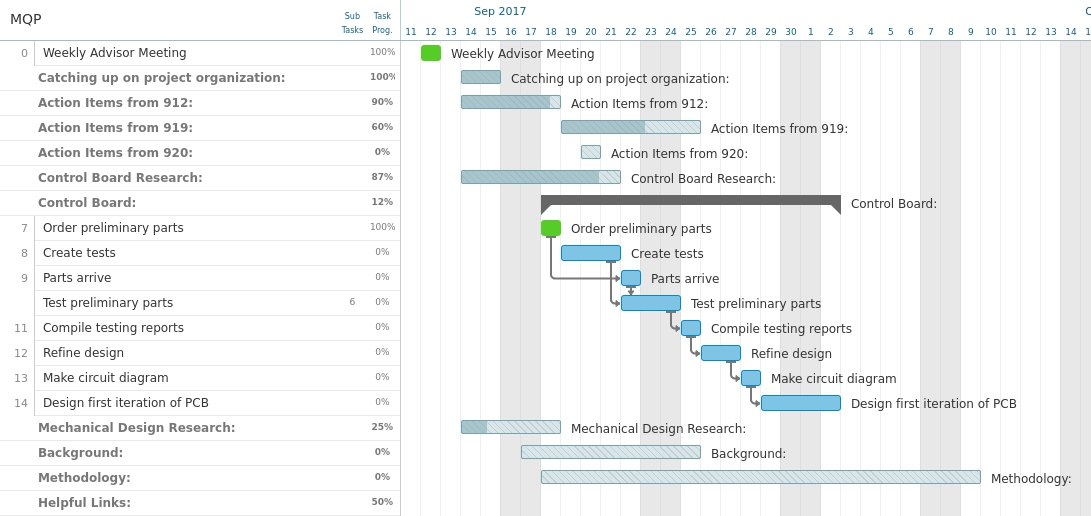
\includegraphics[width=\textwidth]{Gantt_Control_Board}
\caption{Functional block diagram of the system}
\label{fig:Functional_Block_Diagram}
\end{figure}

